\clearpage
\section{Methods}
\label{sec.methods}

% In order to have a quantitative definition of information, three approaches are known: combinatorial, probabilistic and algorithmic~\cite{kolmogorov1965three}, of which probabilistic and algorithmic ones are more popular. By the algorithmic approach, which is followed up by, e.g., Zenil \textit{et~al} in~\cite{zenil2018decomposition,zenil2018algorithmic,soler2017computable}, algorithmic complexity can be approximated based upon the theory of algorithmic probability, namely by the coding theorem method (CTM) and block decomposition method (BDM). In this paper, we follow a combination of probabilistic and algorithmic approaches, although it has a closer connection to the probabilistic one. The proposed amino acid compression method, AC, is based upon a cooperation between finite-context models (FCMs)~\cite{pinho2011representability,pinho2013mfcompress} and substitutional tolerant Markov models (STMMs)~\cite{pratas2016efficient,pratas2017substitutional}. The FCMs follow the probabilistic approach by computing the probability of the next symbol in a sequence, considering the $k$ most recent symbols. This is while the STMMs tend to follow the algorithmic approach by being enabled/disabled based on their performance. It is worth mentioning that the proposed method has been partially published in~\cite{pratas2018compression}. The current paper provides an extensive description of the method along with the results of additional and brand-new experiments. 

% In the following sections, we describe the AC method in great detail. Then, we compare the results of running AC and other compressors on a collection of sequences from several domains and kingdoms. Finally, we present an analysis based on the results of carrying out our compressor on a large collection of reference proteomes.


% % \section{Method} \label{meth}
% AC is based on cooperation between finite-context models and substitutional tolerant Markov models with several depths. The mixture weights associated with each model are updated based on its performance, which is related to the specific forgetting function of each model.


% \subsection{Finite-context models} \label{fcm}
% A finite-context model, relying on the Markov property, considers the $k$ most recent symbols  of an information source (context size of $k$) in order to estimate the probability of the next symbol~\cite{sayood2017introduction,pinho2011representability,pinho2013mfcompress}. Denoting the $k$ most recent symbols as $x_{i-k}^{i-1} = x_{i-k} x_{i-k+1}\cdots x_{i-1}$, the probability of the next symbol $s$, in the position $i$, is estimated as
% \begin{equation} \label{eq:estimate}
% P_m(s|x_{i-k}^{i-1}) = \frac{N(s|x_{i-k}^{i-1})+\alpha}{N(x_{i-k}^{i-1})+ \alpha|\Theta|},
% \end{equation}
% in which $m$ denotes the context model, $N(s|x_{i-k}^{i-1})$ represents the number of times that the information source has generated symbol $s$ in the past, $\Theta$ is the alphabet and $N(x_{i-k}^{i-1}) = \sum_{j \in \Theta} N(j|x_{i-k}^{i-1})$ denotes the total number of events occurred associated with the context~$x_{i-k}^{i-1}$. The parameter $\alpha$ allows balancing between the maximum likelihood estimator and a uniform distribution. Note, for large number of events $i$, the estimator behaves as a maximum likelihood estimator. Also, for $\alpha=1$, Eq.~\ref{eq:estimate} turns to the Laplace estimator~\cite{pratas2015alignment}.

% \subsection{Substitutional tolerant Markov models} \label{stmm}
% A substitutional tolerant Markov model (STMM) \cite{pratas2016efficient,pratas2017substitutional} is a probabilistic-algorithmic context model. 
% An\linebreak STMM uses the occurrence probabilities stored in the memory and assumes that the symbol to be seen in the sequence is the one with the highest probability. This way, it does not take into consideration the symbol that actually is in the sequence. 

% Considering the $k$ most recent symbols, the probability of the next symbol $s$ is estimated as
% \begin{equation}
% P_m(s|{x'}_{i-k}^{i-1}) = \frac{N(s|{x'}_{i-k}^{i-1})+\alpha}
% {N({x'}_{i-k}^{i-1})+ \alpha|\Theta|},
% \end{equation}
% in which $N$ is the memory counts regarding the model and $x'$ is a copy of the context $x$ that is modified as 
% \begin{equation}
% {x'}_{i} = \argmax_{\forall s \in \Theta}{P_m(s|{x'}_{i-k}^{i-1})}.
% \end{equation}

% An STMM is an algorithmic model, namely because it can be disabled and enabled based on its performance. This operation is done considering a predefined threshold $t$. For this purpose, a cache array (history) with the size of $k$ (context-order size) is used to store the recent $k$ hits/misses. When we see a symbol in the sequence, if it is the most probable symbol, based on the number of occurrences saved in the memory, a hit will be stored in the history array; otherwise, a miss will be stored. At the time of seeing a symbol, before storing any hit/miss in the history, we check the number of misses. If it is greater than the threshold $t$, the STMM will be disabled and the history will be reset. This process starts over again for the next symbol.

% To make the difference of FCM and STMM clearer, we give an example. Assume, the current context is\linebreak $c_0=\textrm{FDCAE}$, with $k=5$, and the number of occurrences stored in the memory are $\textrm{F}=8$, $\textrm{D}=5$, $\textrm{C}=12$, $\textrm{A}=7$ and $\textrm{E}=10$. Also, assume the next symbol in the sequence, which is to be compressed, is $\textrm{A}$. Based on an FCM, the next context will be $c_1=\textrm{DCAEA}$, while based on an STMM, it will be $c'_1=\textrm{DCAEC}$. This is because an FCM considers the next symbol as the actual one seen in the sequence, i.e. $\textrm{A}$, but an STMM considers it as the most probable symbol, $\textrm{C}$. This way, the STMM assumes the next symbol to be compressed is $\textrm{C}$, instead of $\textrm{A}$.

% \subsection{Cooperation of FCMs and STMMs} \label{cooper}
% In the case of cooperation between FCMs and STMMs, considering the $k$ most recent symbols in the sequence, the probability of the next symbol $s$ is estimated as
% \begin{equation}
% P(s) = \sum_{m\in\mathcal{F}} P_m(s|x_{i-k}^{i-1})\;w_{m,i} + \sum_{m\in\mathcal{S}} P_m(s|{x'}_{i-k}^{i-1})\;w_{m,i},
% \end{equation}
% where $\mathcal{F}$ is the set of FCMs and $\mathcal{S}$ is the set of STMMs. $P_m(s|x_{i-k}^{i-1})$ and $P_m(s|{x'}_{i-k}^{i-1})$ are the probabilities of the next symbol estimated by the FCM and the STMM, respectively. Also, $w_{m,i}$ is a weight assigned to each model, based on its performance. For this weighting factor, we have
% \begin{align}
% &\forall m\in\mathcal{F}:\quad w_{m,i} \propto (w_{m,i-1})^{\gamma_m} P_m(s | x_{i-k-1}^{i-2})
% \nonumber
% \\[1mm]
% &\forall m\in\mathcal{S}:\quad w_{m,i} \propto (w_{m,i-1})^{\gamma_m} P_m(s | {x'}_{i-k-1}^{i-2}),
% \end{align}
% in which $\gamma_m \in [0,1)$ acts as a forgetting factor for the models. Note,
% \begin{equation}
% \sum_{m\in\mathcal{F}} w_{m,i} + \sum_{m\in\mathcal{S}} w_{m,i} = 1.
% \end{equation}
% We have found that the lower the context-order size $k$, the lower $\gamma_m$ should be assigned to the model, and vice~versa. For example, for a model with $k=6$, a $\gamma_m \simeq 0.9$ and for a model with $k=18$, a $\gamma_m \simeq 0.95$ is the appropriate choice. This means, the more complex the model, the less the forgetting intensity.



The schema of the proposed method is illustrated in Fig.~\ref{fig.schema}. There are five major stages in this method, including 

\begin{figure}[!h]
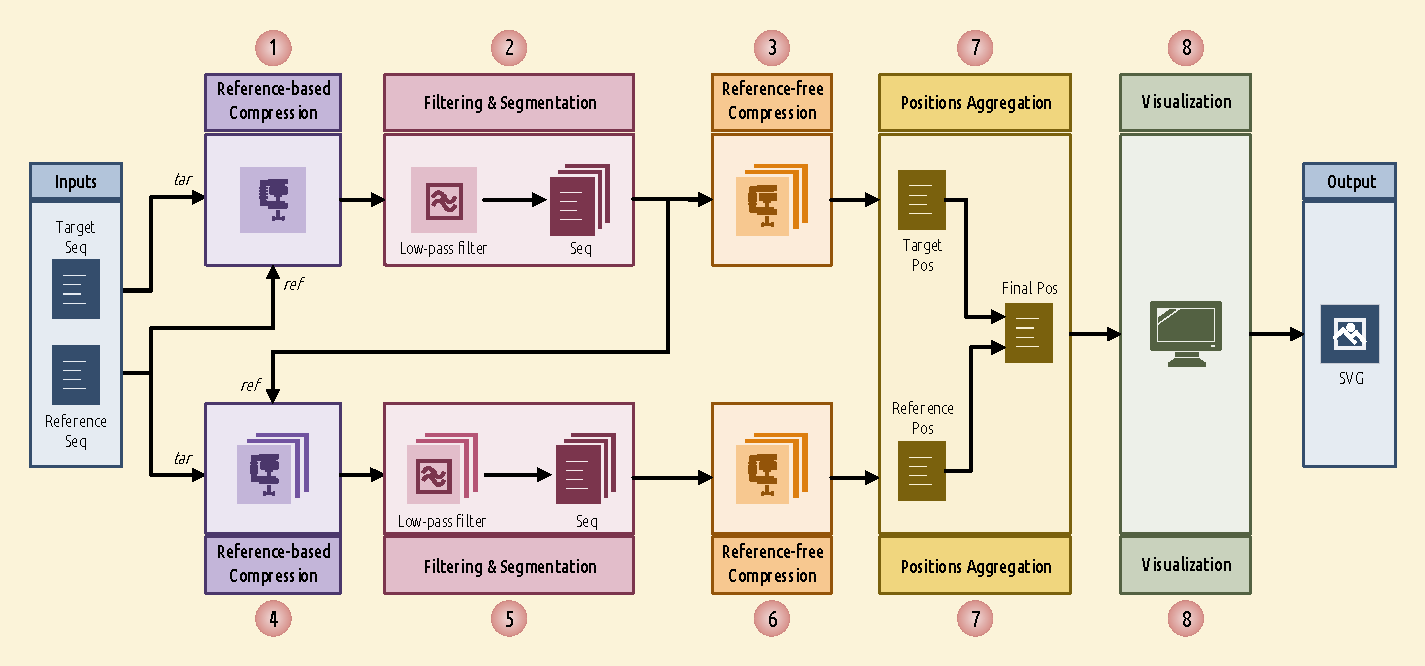
\includegraphics[width=\linewidth]{schema.pdf}
\caption{The schema of Smash++.}
\label{fig.schema}
\end{figure}

\subsection{Building models of the data}

\subsection{finding similar regions}

In order to smooth the profile information, we use Hann window~\cite{blackman1959particular}, which is a discrete window function given by
\begin{equation}
  \label{eq.hann}
  w[n]=0.5-0.5\;\cos \left({\frac {2\pi n}{N}}\right)=\sin ^{2}\left({\frac {\pi n}{N}}\right),
\end{equation}
in which, $0\le n\le N$ and length of the window is $N+1$ (Fig.~\ref{fig.hann}).

\begin{figure}[!h]
  \centering
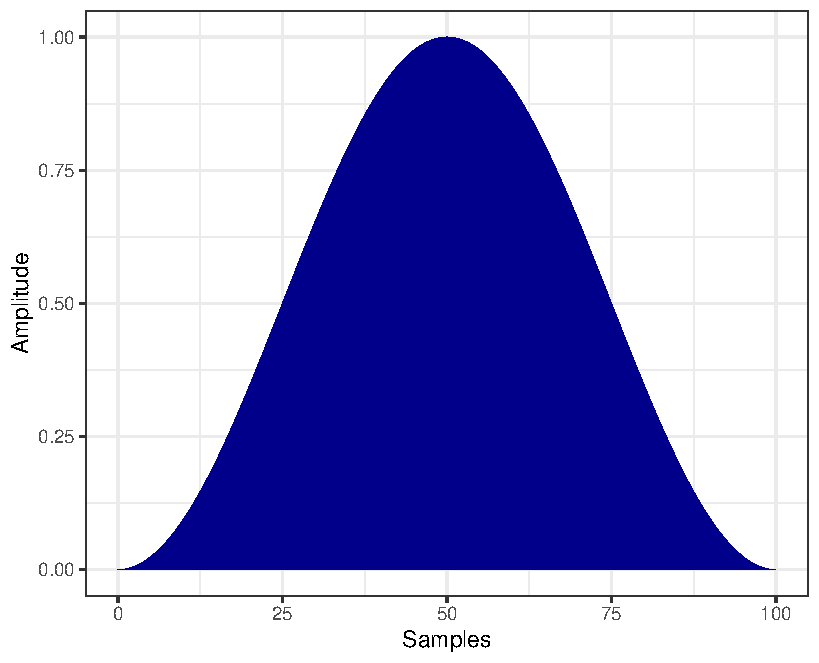
\includegraphics[width=7cm]{hann.pdf}
\caption{Hann window for 101 samples.}
\label{fig.hann}
\end{figure}

\subsection{Computing complexities}

\subsection{The software}

Besides Hann window, that is used as default to filter the profile information obtained by the reference-based compression, we have implemented several other window functions (Fig.~\ref{fig.filters}), including Blackman~\cite{blackman1959particular}, Hamming~\cite{tukey1949measuring}, Nuttall~\cite{nuttall1981some}, rectangular~\cite{oppenheim1999discrete}, sine~\cite{harris1978use}, triangular~\cite{bartlett1950periodogram} and Welch~\cite{welch1967use} windows. These functions are given by
\begin{align}
  w[n] &= 1,
  \tag*{(rectangular)} \\
  w[n] &= 1-\left|\tfrac {n-N/2}{L/2}\right|, \quad L=N,
  \tag*{(triangular/Bartlett)} \\
  w[n] &= 1-\left(\tfrac {n-N/2}{N/2}\right)^{2},
  \tag*{(Welch)} \\
  w[n] &= \sin \left(\tfrac {\pi n}{N}\right),
  \tag*{(sine)} \\
  w[n] &= 0.54348-0.45652\;\cos \left(\tfrac {2\pi n}{N}\right),
  \tag*{(Hamming)} \\
  w[n] &= 0.42659-0.49656\;\cos \left(\tfrac {2\pi n}{N}\right)+0.07685\;\cos \left(\tfrac {4\pi n}{N}\right),
  \tag*{(Blackman)} \\
  w[n] &= 0.35577-0.48740\;\cos \left(\tfrac {2\pi n}{N}\right)+0.14423\;\cos \left(\tfrac {4\pi n}{N}\right)-0.01260\;\cos \left(\tfrac {6\pi n}{N}\right).
  \tag*{(Nuttall)} \\
\end{align}

\begin{figure}[!h]
  \centering
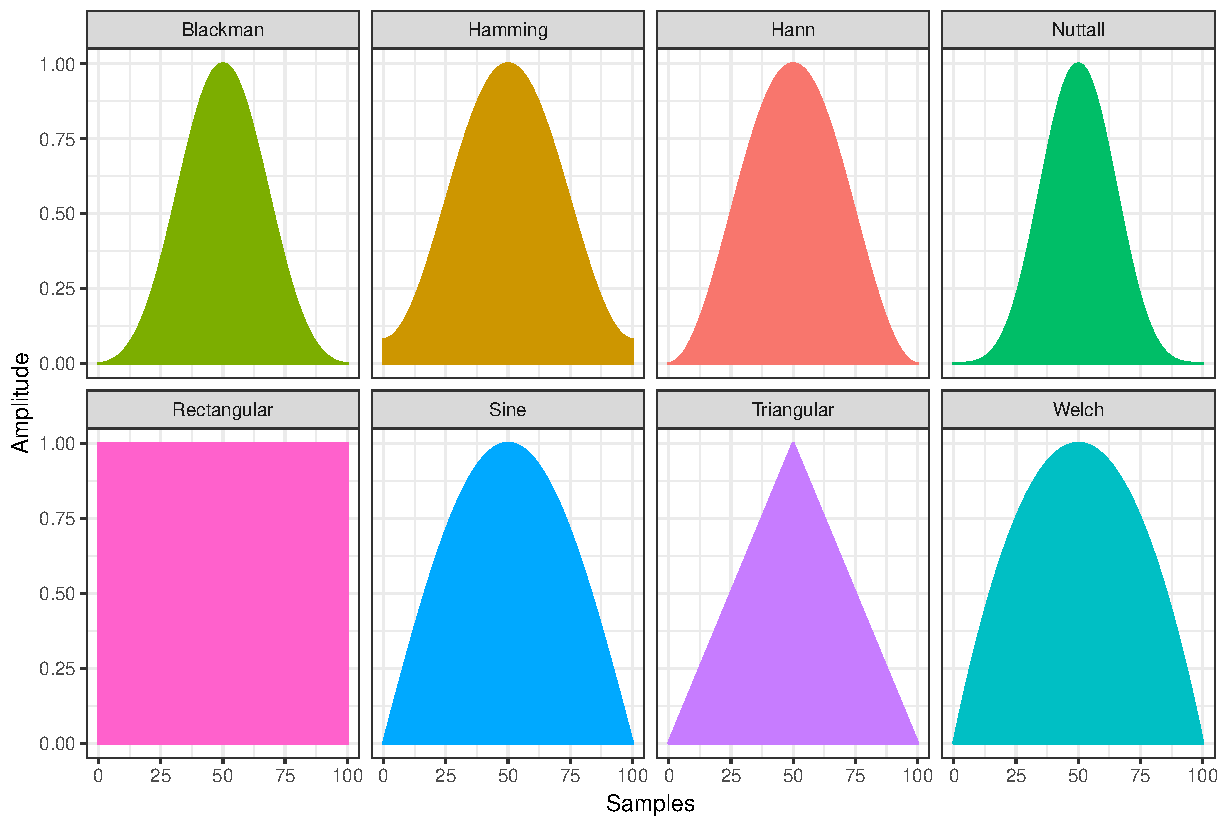
\includegraphics[width=.95\linewidth]{filters.pdf}
\caption{Window functions.}
\label{fig.filters}
\end{figure}